\documentclass[12pt]{article}

\usepackage{amsmath}
\usepackage{graphicx}
\usepackage{hyperref}
\usepackage{amsfonts}
\usepackage{fullpage}
\usepackage{booktabs}
\usepackage{tabularx} % Resizable tabular environment

\newcommand{\mname}[1]{\mbox{\sf #1}}

\pagestyle{plain}
\pagenumbering{arabic}

\newcounter{stepnum}

%%%%%%%%%%%%%%%
% The environment below is used for text file extension Verbatim inclusion
%%%%%%%%%%%%%%%
\usepackage[dvipsnames]{xcolor}

\usepackage{fancyvrb}

% redefine \VerbatimInput
\RecustomVerbatimCommand{\VerbatimInput}{VerbatimInput}%
{fontsize=\footnotesize,
 %
 frame=lines,  % top and bottom rule only
 framesep=2em, % separation between frame and text
 rulecolor=\color{Gray},
 %
 label=\fbox{\color{Black}Revision History},
 labelposition=topline,
 %
 commandchars=\|\(\), % escape character and argument delimiters for
                      % commands within the verbatim
 commentchar=*        % comment character
}

\begin{document}

\begin{titlepage} % Suppresses headers and footers on the title page

	\centering % Centre everything on the title page
	
	\scshape % Use small caps for all text on the title page
	
	\vspace*{\baselineskip} % White space at the top of the page
	
	%------------------------------------------------
	%	Title
	%------------------------------------------------
	
	\rule{\textwidth}{1.6pt}\vspace*{-\baselineskip}\vspace*{2pt} % Thick horizontal rule
	\rule{\textwidth}{0.4pt} % Thin horizontal rule
	
	\vspace{0.75\baselineskip} % Whitespace above the title
	
	{\LARGE SE2XB3 OptimizeU V1.0 \\ Design Specification\\} % Title
	
	\vspace{0.75\baselineskip} % Whitespace below the title
	
	\rule{\textwidth}{0.4pt}\vspace*{-\baselineskip}\vspace{3.2pt} % Thin horizontal rule
	\rule{\textwidth}{1.6pt} % Thick horizontal rule
	
	\vspace{2\baselineskip} % Whitespace after the title block
	
	%------------------------------------------------
	%	Subtitle
	%------------------------------------------------
	
	Final Project for SFWRENG 2XB3:Software Engineering Practice and Experience: 
	Binding Theory to Practice
	
	\vspace*{3\baselineskip} % Whitespace under the subtitle
	
	%------------------------------------------------
	%	Group members
	%------------------------------------------------
	
	Group 8\\ Members:\\
	
	\vspace{0.5\baselineskip}
	
	{\scshape\Large Lucas Matthew Dutton \\ Michael Le \\ Saad Khan \\ Omar Elemary\\}
	
	\vspace{0.5\baselineskip} 
	
	\textit{McMaster University \\ Department of Computing and Software} 
	
	\vfill
	
	%------------------------------------------------
	%	Date
	%------------------------------------------------
	
	Created and Edited on: April 1, 2018 

\end{titlepage}

\tableofcontents

\newpage

\section{Revisions}

\subsection{Revision History}

\VerbatimInput{log.txt}

\newpage

\subsection{Team Details}

\begin{table}[h]
\begin{tabular}{| l | l | l |}
\hline
\textbf{Name} & \textbf{Student Number} & \textbf{Roles} \\ 
\hline
Michael Le & 400070369 & Group Leader, Graphics Implementation\\ 
\hline
Lucas Dutton & 400052930 & Log Admin, Algorithms Implementation\\ 
\hline
Saad Khan & 400085498 & Documentation Designer, Server Researcher\\ 
\hline
Omar Elemary & 400100169 & Algorithms Researcher, Test\\ 
\hline
\end{tabular}
\end{table}

\subsection{Attestation and Consent}

\textit{By virtue of submitting this document we electronically sign
and date that the work being submitted by all the individuals in the 
group is their exclusive work as a group and we consent to make
available the application developed through SE2XB3 project, the 
reports, presentations and assignments (not including my name or 
student number) for future teaching purposes.}

\newpage

\section{Contributions}
Note: Member roles are outlines in \textbf{Revisions: Team Details}

\begin{table}[h]
\begin{tabularx}{\textwidth}{|l|X|X|}
\hline
\textbf{Name} & \textbf{Contributions} & \textbf{Comments} \\
\hline
Lucas Dutton & Implemented Kruskals, K-Means and Associated ADT
               (Abstract Data Type)
             & Responsible for implementing and updating algorithms
               with any project changes\\
\cline{2-3}
~ & Project Log admin 
  & Responsible for monitoring and approving Project Logs\\
\cline{2-3}
~ & Documentation editor
  & Responsible for creating and sharing documents such as 
    Requirements and Design Specifications\\
\hline
Michael Le & Implemented graphical representation of outputs
           & Responsible for presenting data in a graphical
             environment in Java\\
\cline{2-3}
~ & Implemented graphical ADTs 
  & Cluster and Cord ADTs made for interaction between algorithms
    and graphics\\
\cline{2-3}
~ & Source Code documentation & Comment each methods in each module\\
\hline
Saad Khan & Presentation Facilitator 
          & Responsible for organizing presentation slides\\
\cline{2-3}
~ & Graphics creator for documents 
  & Responsible for creating diagrams for documents, e.g. UML\\
\hline
Omar Elemary & Meeting Minutes upkeep
             & Responsible for creating and updating project logs\\
\cline{2-3}
~ & Unit tester
  & Responsible for testing each modules and the application\\
\hline
\end{tabularx}
\end{table}

\newpage

\section{Executive Summary}
OptimizeU is intended to be a portable app that addresses the problem of finding an Uber pickup
on busy nights, as well as optimizing driving routes of Uber drivers. The project leverages a 
dataset of twenty million Uber pick ups in New York City to help drivers locate the
busiest hotspots in the city, routing more cars to denser locations which allows more users
to find access to an Uber vehicle in a faster time. The application uses various algorithms
related to machine learning and graphing, as well as pre-processing the dataset with searching
and sorting algorithms to generate a pick-up density map of the city. The map will contain
heat clusters related to density and distances between each cluster to inform the driver of
optimal routes that can be taken. In short, the aim of OptimizeU is decrease wait times of
passengers and maximize profits of Uber drivers.

\newpage

\section{Design Description}
\subsection{Module Description and Decomposition}
\subsubsection{Module Overview}
The table below shows a top-level view of each class in the application. Classes are grouped
by their functionality and dependency on one another.
\begin{table}[h]
\begin{tabularx}{\textwidth}{|l|l|X|}
\hline
\textbf{Function} & \textbf{Class Name} & \textbf{Description}\\
\hline
Basic Representation & Cord & 2-Dimensional representation of coordinates\\
\hline
Clustering & Cluster & Representation of a cluster produced by K-Means\\
\cline{2-3}
~ & KMeans & Clustering algorithm API\\
\hline
Minimum Spanning Tree & KruskalMST & Driver class to calculate Minimum
                                     Spanning Tree\\
\cline{2-3}
~ & Edge & ADT representation of weighted edges\\
\cline{2-3}
~ & Graph & Module to instantiate a graph with directed edges\\
\cline{2-3}
~ & UF & Helper module for connecting vertices in a graph\\
\cline{2-3}
~ & Heap & Heapsort on edges for Kruskals\\
\hline
Input/Output & Load & Reads dataset, sorts them according to time,
                      and puts each coordinate in a Hash Table\\
\cline{2-3}
~ & drawSurface & Graphics implementation of clusters and MST\\
\cline{2-3}
~ & demoFrame & Main driver of application\\
\hline
\end{tabularx}
\end{table}

\newpage
\subsubsection{Module Decomposition Semantics}
Following the table in the previous section, the following items below provide a more detailed
description of the rationale behind the modular decomposition of the design.
\begin{itemize}
\item \textbf{Basic Representation:} Since the application makes use of 
coordinates on a two-dimensional plane, the Cord API makes available a 
convenient coordinate ADT that is used whenever a point in the plane needs
to be represented or stored.
\item \textbf{Clustering:} KMeans and its associated ADT, Clusters, are used
to compute clusters from a random number of points. Clusters are stored in the
ADT as a point representing the mean of the cluster, called the centroid.
All points associated to the centroid are stored in the ADT as well
\item \textbf{Minimum Spanning Tree:} Kruskal's algorithm is used to generate
the minimum spanning tree of the clusters' centroids. All the associated modules
are helpers to the algorithm, such as union-find, sorting, and graph/edge
representations.
\item \textbf{Input and Output:} This can be divided by itself into two parts:
input and output. Load is the input routine of the application: It leverages
countsort to sort input data according to the pickup time which is 
partitioned by th 24-hour system. The other two modules are used to collect
output from the algorithms and display it on a graphic canvas.
\end{itemize}

\newpage
\subsubsection{Uses Relation}
An overlay of the application can be viewed in the Uses relationship below:
\begin{figure}[h]
\centering
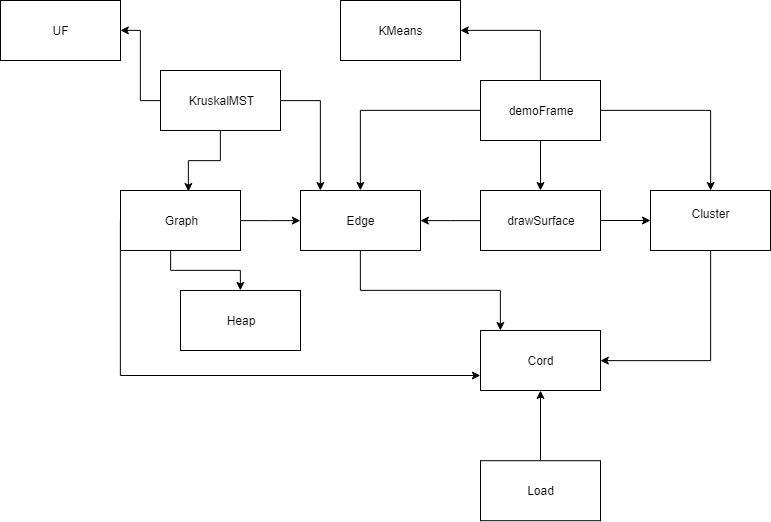
\includegraphics[width=1.0\textwidth]{UsesDiagram.png}
\end{figure}
\newpage

\subsubsection{UML Class Diagram}
An overlay of the application can be viewed in the UML class diagram below:
\begin{figure}[h]
\centering
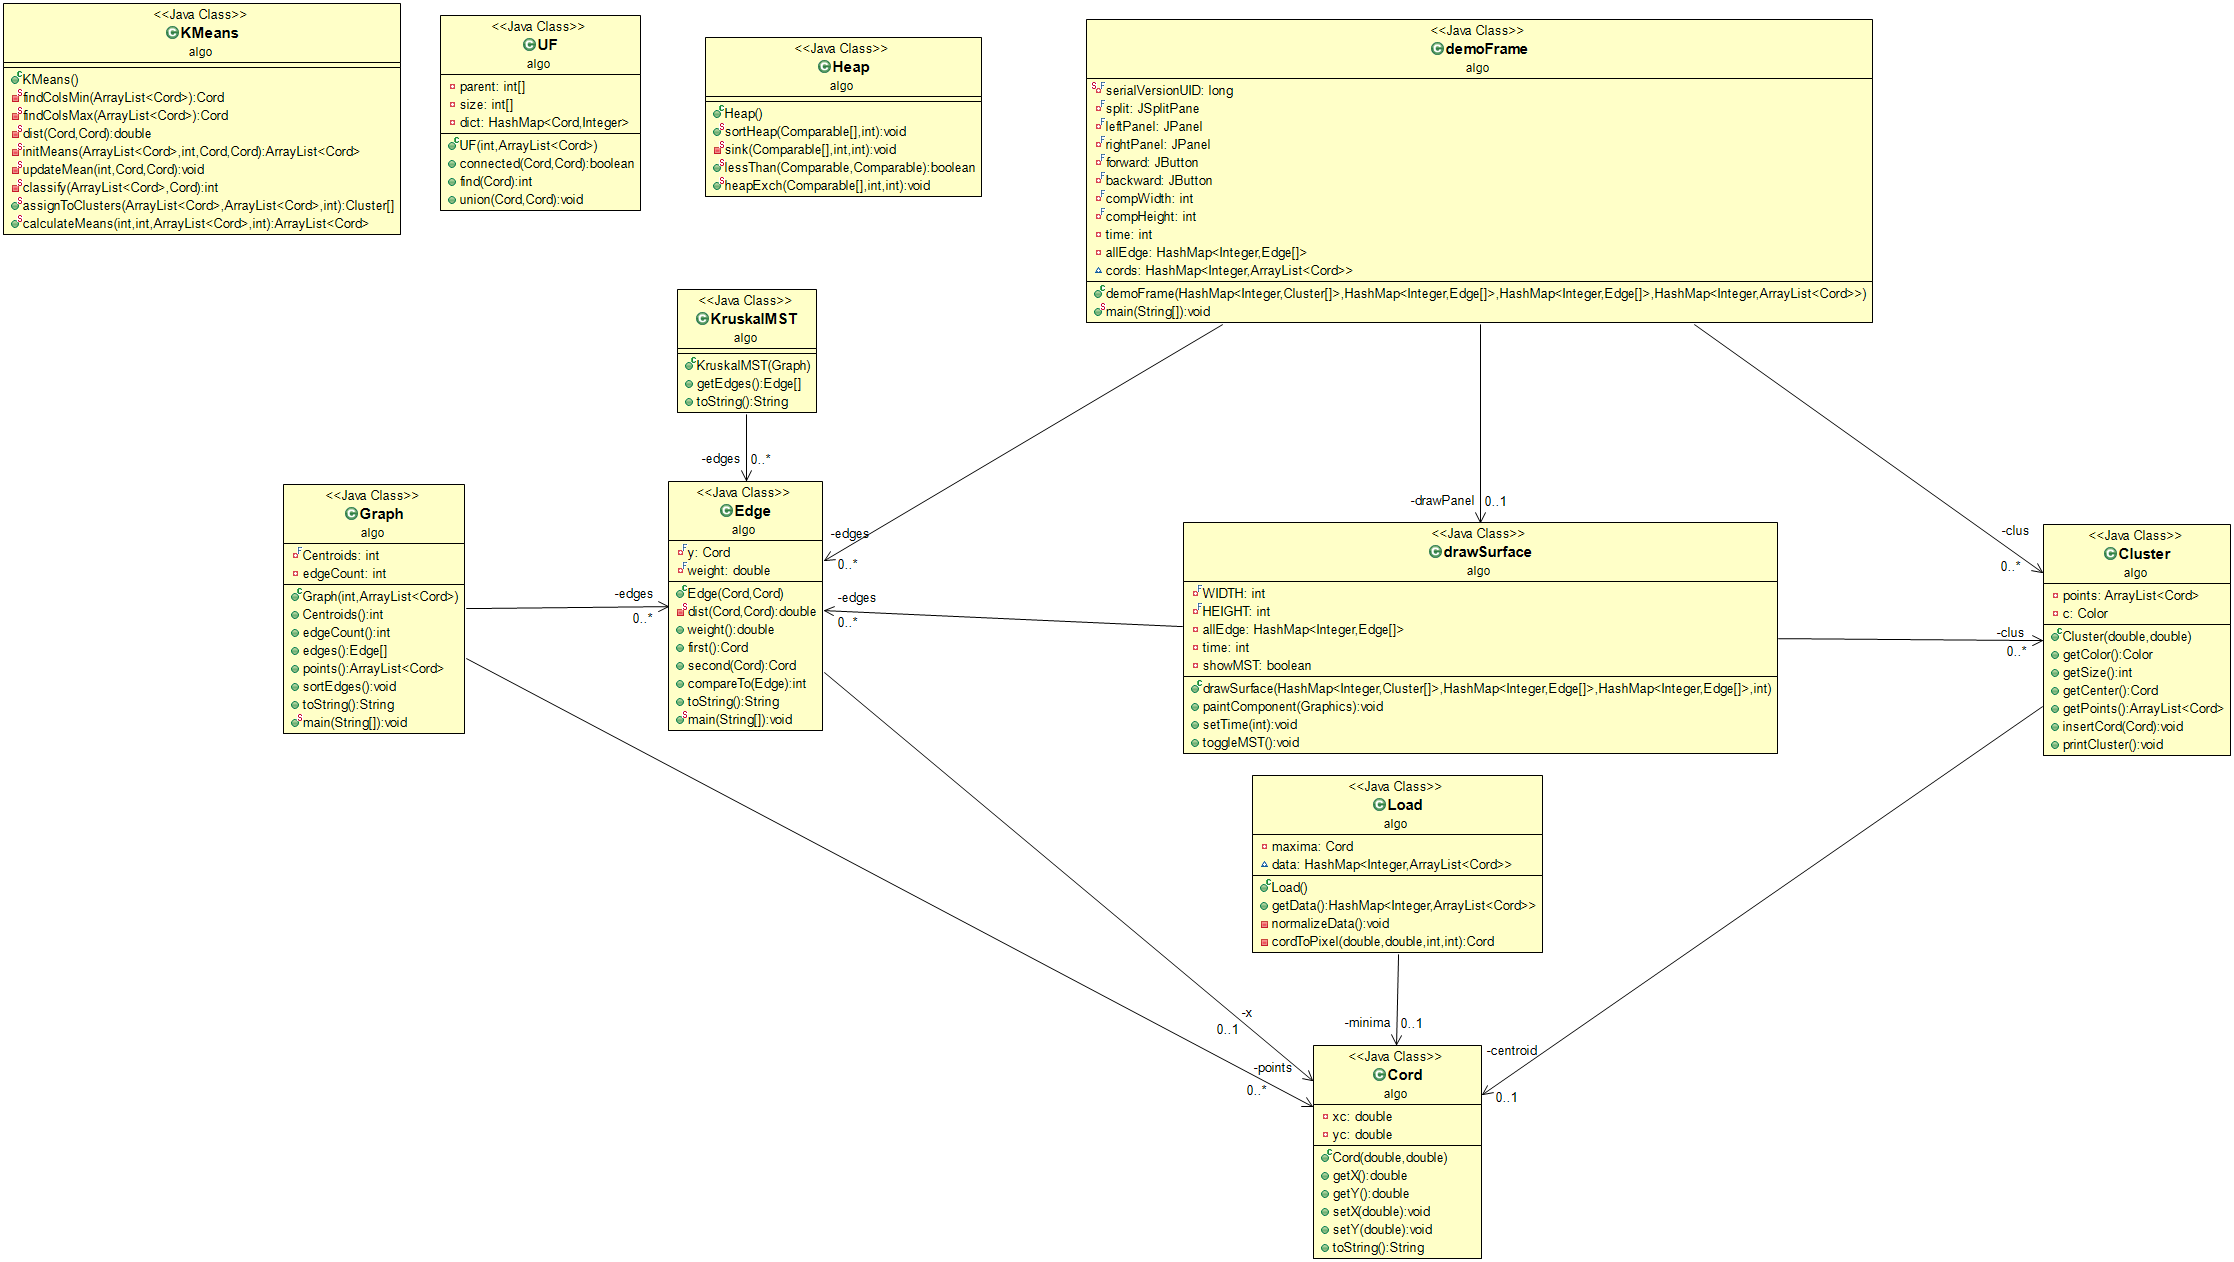
\includegraphics[width=1.0\textwidth]{UML.png}
\end{figure}

\newpage
\subsection{Module Interface Specification}
This section will cover:
\begin{itemize}
\item A description of the interface of each public entity, as well as its syntax
and semantics
\item A description of the implementation of private entities of each module,
state variables and how the methods maintain these state variables
\item Requirements trace back for each module
\end{itemize}

\noindent
Several items should be noted about the module specifications:
\begin{itemize}
\item Where possible, a more formal, mathematical notation similar to conventions 
used in SE2AA4 will be used.
\item A natural language description will be used for methods that are too
complicated or incomprehensible to be expressed with discrete mathematics
\item Each module specification will cover both public and private entities. Care
is taken to seperate between the two for each module to prevent ambiguity issues.
\end{itemize}

\newpage

\section*{Cord Module}

\subsection*{Top Level Description}

An abstract data type to represent a point in a two-dimensional space

\subsection*{Module}

Cord

\subsection* {Uses}

N/A

\subsection* {Syntax}

\subsubsection* {Exported Types}

Cord = ?

\subsubsection* {Exported Access Programs}

\begin{tabular}{| l | l | l |}
\hline
\textbf{Routine name} & \textbf{In} & \textbf{Out}\\
\hline
Cord & $\mathbb{R}$, $\mathbb{R}$ & Cord\\
\hline
getX & ~ & $\mathbb{R}$\\
\hline
getY & ~ & $\mathbb{R}$\\
\hline
setX & $\mathbb{R}$ & ~\\
\hline
setY & $\mathbb{R}$ & ~\\
\hline
toString & ~ & String \\
\hline
\end{tabular}

\subsection* {Semantics}

\subsubsection* {State Variables}

$xc$: $\mathbb{R}$\\
$yc$: $\mathbb{R}$

\subsubsection* {State Invariant}

None

\subsubsection* {Access Routine Semantics}

Cord($x$,$y$):\\
\textit{Constructor for a coordinate point in a 2D-plane}
\begin{itemize}
\item transition: $xc, yc := x, y$
\item output: $out := \mathit{self}$
\end{itemize}

\noindent
getX():\\
\textit{Accessor for the x-coordinate}
\begin{itemize}
\item output: $out := xc$
\end{itemize}

\noindent
getY():\\
\textit{Accessor for the y-coordinate}
\begin{itemize}
\item output: $out := yc$
\end{itemize}

\noindent
setX(x):\\
\textit{Mutator for the x-coordinate}
\begin{itemize}
\item transition: $xc := x$
\item output: None
\end{itemize}

\noindent
setY(y):\\
\textit{Mutator for the y-coordinate}
\begin{itemize}
\item transition: $yc := y$
\item output: None
\end{itemize}

\noindent
toString():\\
\textit{Override for Java method toString. Represents a coordinate in the
form of a string "(x,y)" where x and y are xc and yc respectively}.

\newpage
%%%%%%%%%%%%%%%%%%%%%%%%%%%%%%%%%%%%%%%%%%%%%%%%%%%%%%%%%%%%%%%%%%%%%%%%%%

\section*{Cluster Module}

\subsection* {Top Level Description}

Stores the centroid of a clusters and points associated with the cluster.

\subsection*{Module}

Cluster

\subsection* {Uses}

Cord, Color, ArrayList

\subsection* {Syntax}

\subsubsection* {Exported Types}

Cluster = ?

\subsubsection* {Exported Access Programs}

\begin{tabular}{| l | l | l |}
\hline
\textbf{Routine name} & \textbf{In} & \textbf{Out}\\
\hline
Cluster & $\mathbb{R}$, $\mathbb{R}$ & Cluster\\
\hline
getColor & ~ & $Color$\\
\hline
getSize & ~ & $\mathbb{N}$\\
\hline
getCenter & ~ & Cord \\
\hline
getPoints & ~ & sequence of Cord\\
\hline
insertCord & Cord & ~ \\
\hline
printCluster & ~ & ~ \\
\hline
\end{tabular}

\subsection* {Semantics}

\subsubsection* {State Variables}
centroid: Cord\\
points: seq of Cord\\
c: Color

\subsubsection* {State Invariant}

None

\subsubsection* {Assumptions}
\begin{itemize}
\item c : Color represents the color of the cluster when drawn with Java's graphics
library
\item centroid represents a Cluster's centroid
\item points represents the Cord points associated with the centroid
\end{itemize}

\subsubsection* {Access Routine Semantics}

Cluster(x,y):\\
\textit{Constructor for Cluster Object}
\begin{itemize}
\item transition: points, centroid, c $:=  <>, \mbox{Cord}(x,y), \mbox{random Color}$
\item output: $out := \mathit{self}$
\end{itemize}

\noindent
getColor():\\
\textit{Return the color of the cluster}
\begin{itemize}
\item output: $out := c$
\end{itemize}

\noindent
getSize():\\
\textit{Return the number of points associated with the cluster}
\begin{itemize}
\item output: $out := |\mbox{points}|$
\end{itemize}

\noindent
getCenter():\\
\textit{Returns the Cord representing the centroid}
\begin{itemize}
\item output: $out := \mbox{centroid}$
\end{itemize}

\noindent
getPoints():\\
\textit{Returns the sequence of points associated to the cluster}
\begin{itemize}
\item output: $out := \mbox{points}$
\end{itemize}

\noindent
insertCord(n):\\
\textit{Insert a point into the sequence of Cord, associating the inserted
point with the cluster}
\begin{itemize}
\item transition: $\mbox{points} := \mbox{points} || n$
\item output: None
\end{itemize}

\noindent
printCluster():\\
\textit{Prints each Cord object in the sequence of coordinates}

\newpage
%%%%%%%%%%%%%%%%%%%%%%%%%%%%%%%%%%%%%%%%%%%%%%%%%%%%%%%%%%%%%%%%%%%%%%%%%%%%%%%

\section*{KMeans Library Module}

\subsection* {Top Level Description}

A module that clusters points using K-Means classification

\subsection*{Module}

KMeans

\subsection* {Uses}

Cord, Cluster

\subsection* {Syntax}

\subsubsection* {Exported Types}

KMeans = ?

\subsubsection* {Exported Access Programs}

\begin{tabular}{| l | l | l |}
\hline
\textbf{Routine name} & \textbf{In} & \textbf{Out}\\
\hline
calculateMeans & $\mathbb{N}, \mathbb{N}, \mathbb{N}$, seq of Cord & seq of Cord\\
\hline
assignToClusters & seq of Cord, seq of Cord, $\mathbb{N}$ & seq of Cluster\\
\hline
\end{tabular}

\subsubsection* {Private Access Programs}

\begin{tabular}{| l | l | l |}
\hline
\textbf{Routine name} & \textbf{In} & \textbf{Out}\\
\hline
findColsMin & seq of Cord & Cord\\
\hline
findColsMax & seq of Cord & Cord\\
\hline
dist & Cord, Cord & $\mathbb{R}$ \\
\hline
updateMean & $\mathbb{N}$, Cord, Cord & ~ \\
\hline
classify & seq of Cord, Cord & $\mathbb{N}$ \\
\hline
\end{tabular}

\subsection* {Semantics}

\subsubsection* {State Variables}

None

\subsubsection* {State Invariant}

None

\subsubsection* {Assumptions}

\begin{itemize}
\item calculateMeans is called to obtain cluster centroids before a call
to assignToClusters.
\item Cluster sizes remain consistent between the two method calls.
\end{itemize}

\subsubsection* {Access Routine Semantics}

calculateMeans(k, datasize, maxIterations, items :: seq of Cord):\\
KMeans Clustering heuristic. Takes as input:
\begin{itemize}
\item k: The amount of clusters to generate
\item datasize: The size of the input data
\item maxIterations: Loop termination count, in the event that the
heuristic is non-deterministic.
\item items: The input data of Cords as a sequence
\end{itemize}
\noindent
Returns as output a set of cluster centroids as calculated from the 
input parameters.\\

\noindent
assignToClusters(means, items, k : $\mathbb{N}$):\\
Associate each input point with centroids calculated from calculateMeans.
Takes as input:
\begin{itemize}
\item k: The amount of clusters to generate
\item means: The centroids generated from calculateMeans
\item items: The input points
\end{itemize}
Returns as output a sequence of Cluster objects, each representing
points associated to a centroid.

\subsubsection* {Private Routine Semantics}
findColsMin(items):\\
\textit{Output the point denoting the bottom left of the map used to calculate clusters}
\begin{itemize}
\item output: $out := \exists (c : \mbox{Cord} | c \in \mbox{items} \land
                      \forall (n : \mathbb{N} | n \in [0..|\mbox{items}|-1] :
                      c \leq \mbox{items}[n]) : c)$
\end{itemize}

\noindent
findColsMan(items):
\textit{Output the point denoting the bottom left of the map used to calculate clusters}
\begin{itemize}
\item output: $out := \exists (c : \mbox{Cord} | c \in \mbox{items} \land
                      \forall (n : \mathbb{N} | n \in [0..|\mbox{items}|-1] : 
                      c \geq \mbox{items}[n]) : c)$
\end{itemize}

\noindent
dist($a$, $b$):
\textit{Compute the Euclidean distance between two coordinates}
\begin{itemize}
\item output: $out := \sqrt{(b.xc-a.xc)^{2} + (b.yc-a.yc)^{2}}$
\end{itemize}

\noindent
updateMean(size : $\mathbb{N}$, mean, item):\\
\textit{Updates the mean centroid after adding associating an additonal point to it}
\begin{itemize}
\item transition: $mean := (\mbox{mean}*(\mbox{size}-1) + \mbox{item})/\mbox{size}$
\item output: None
\end{itemize}

\noindent
classify(means, item : Cord):\\
\textit{Classifies a point to the nearest centroid, returns the index in which the
point is associated to in the sequence of centroids}

\newpage
%%%%%%%%%%%%%%%%%%%%%%%%%%%%%%%%%%%%%%%%%%%%%%%%%%%%%%%%%%%%%%%%%%%%%%%%%%%%%%%

\section*{Edge Module}

\subsection* {Top Level Description}

An object representing weighted edges in a two-dimensional graph

\subsection*{Module}

Edge

\subsection* {Uses}

Cord

\subsection* {Syntax}

\subsubsection* {Exported Types}

Cord = ?

\subsubsection* {Exported Access Programs}

\begin{tabular}{| l | l | l |}
\hline
\textbf{Routine name} & \textbf{In} & \textbf{Out}\\
\hline
Edge & Cord, Cord & Edge\\
\hline
weight & ~ & $\mathbb{R}$\\
\hline
first & ~ & Cord \\
\hline
second & Cord & Cord\\
\hline
compareTo & Edge & $\mathbb{Z}$\\
\hline
toString & ~ & String\\
\hline
\end{tabular}

\subsubsection* {Private Access Programs}

\begin{tabular}{| l | l | l |}
\hline
\textbf{Routine name} & \textbf{In} & \textbf{Out}\\
\hline
dist & Cord, Cord & $\mathbb{R}$ \\
\hline
\end{tabular}

\subsection* {Semantics}

\subsubsection* {State Variables}

$x$: Cord\\
$y$: Cord\\
weight: $\mathbb{R}$

\subsubsection* {State Invariant}

None

\subsubsection* {Access Routine Semantics}

Edge(X,Y):\\
\textit{Constructor of an Edge object}
\begin{itemize}
\item transition: $x, y, weight := X, Y, dist(X,Y)$
\item output: $out := \mathit{self}$
\end{itemize}

\noindent
weight():\\
\textit{Accessor for the weight of the edge}
\begin{itemize}
\item output: $out := weight$
\end{itemize}

\noindent
first():\\
\textit{Returns the point stored in the state variable x}
\begin{itemize}
\item output: $out := x$
\end{itemize}

\noindent
second(point):\\
\textit{Returns the point that connects from the input point}
\begin{itemize}
\item output: $out := point = \mbox{point} = y \Rightarrow x | \mbox{point} = x \Rightarrow y$
\item exception: $exc := point \neq x \lor y \Rightarrow IllegalArgumentException$
\end{itemize}

\noindent
compareTo(that):\\
\textit{Implemens compareTo for Java's comparable interface. Used for sorting edges by weight.}
\begin{itemize}
\item output: \\\\
\begin{tabular}{| l | l |}
\hline
\textbf{Condition} & \textit{out}\\
\hline
weight $<$ that.weight & -1 \\
\hline
weight $>$ that.weight & 1 \\
\hline
weight $\equiv$ that.weight & 0 \\
\hline
\end{tabular}
\end{itemize}

\noindent
toString():\\
\textit{Java override of toString method. Prints the details of the Edge object}

\subsubsection* {Private Routine Semantics}
dist($a$, $b$):
\textit{Compute the Euclidean distance between two coordinates. Used for calculating the weight
of the edge}
\begin{itemize}
\item output: $out := \sqrt{(b.xc-a.xc)^{2} + (b.yc-a.yc)^{2}}$
\end{itemize}

\newpage
%%%%%%%%%%%%%%%%%%%%%%%%%%%%%%%%%%%%%%%%%%%%%%%%%%%%%%%%%%%%%%%%%%%%%%%%%%%%%%%

\section*{Heap Library Module}

\subsection* {Top Level Description}

Heapsorts an array of Comparable Objects. Used in KruskalMST to sort an array of Edges.

\subsection*{Module}

Heap

\subsection* {Uses}

None

\subsection* {Syntax}

\subsubsection* {Exported Types}

Heap = ?

\subsubsection* {Exported Access Programs}

\begin{tabular}{| l | l | l | l |}
\hline
\textbf{Routine name} & \textbf{In} & \textbf{Out}\\
\hline
sortHeap & seq of Comparable, $\mathbb{N}$ & ~ \\
\hline
\end{tabular}

\subsubsection* {Private Access Programs}

\begin{tabular}{| l | l | l |}
\hline
\textbf{Routine name} & \textbf{In} & \textbf{Out}\\
\hline
sink & seq of Comparable, $\mathbb{N}, \mathbb{N}$ & ~ \\
\hline
lessThan & Comparable, Comparable, & $\mathbb{B}$ \\
\hline
heapExch & seq of Comparable, $\mathbb{N}, \mathbb{N}$ & ~ \\
\hline
\end{tabular}

\subsection* {Semantics}

\subsubsection* {State Variables}

None
\subsubsection* {State Invariant}

None

\subsubsection* {Access Routine Semantics}

sortHeap($x$ : seq of Comparable, $n$ : $\mathbb{N}$):\\\\
Calls heapsort on the array $x$ of size $n$. The process is twofold:
\begin{enumerate}
\item Builds the heap from the array. The array will obey the max heap property
      after this process terminates
\item Sorts the array using $n$ extractMaxes
\end{enumerate}

\noindent
Formally, sortHeap produces an output array which satisfies the following property:\\

$\forall (n : \mathbb{N} | n \in [1..|x|-1] : x[n] \geq x[n-1])$\\

\noindent
sortHeap happens in-place, which is important in this application as processing a large
dataset may constrain available memory.

\subsubsection* {Private Routine Semantics}

sink($x$ : seq of Comparable, $n$ : $\mathbb{N}$, length : $\mathbb{N}$):\\
A helper function used to sink elements in a heap. Takes as input:
\begin{itemize}
\item $x$: an array of Comparable objects
\item $n$: The index of the element to sink
\item length: The size of x
\end{itemize}
This function is used to fix any violations in the max heap property.\\

\noindent
lessThan(a, b):\\
\textit{Compares a and b using Java's compareTo implementation}\\

\noindent
heapExch($arr$, $i$ ,$j$):\\
\textit{Swaps elements at index i and j. This accounts for heaps having 1-index starts}
\begin{itemize}
\item transition: $arr[i-1], arr[j-1] := arr[j-1], arr[i-1]$
\end{itemize}

\newpage

%%%%%%%%%%%%%%%%%%%%%%%%%%%%%%%%%%%%%%%%%%%%%%%%%%%%%%%%%%%%%%%%%%%%%%%%%%%%%%%

\section*{Graph Module}

\subsection* {Top Level Description}

Representation of a directed graph, in the specific application domain of representing
the output of clustering with K-Means using cluster centroids as nodes and edges as
the connection between each point.

\subsection*{Module}

Graph

\subsection* {Uses}

Edge, Cord, ArrayList

\subsection* {Syntax}

\subsubsection* {Exported Types}

Graph = ?

\subsubsection* {Exported Access Programs}

\begin{tabular}{| l | l | l |}
\hline
\textbf{Routine name} & \textbf{In} & \textbf{Out}\\
\hline
Graph & $\mathbb{N}$, seq of Cord & Graph\\
\hline
centroids & ~ & $\mathbb{N}$\\
\hline
edgeCount & ~ & $\mathbb{N}$\\
\hline
edges & ~ & seq of Edge\\
\hline
points & ~ & seq of Cord \\
\hline
sortEdges & ~ & ~ \\
\hline
toString & ~ & ~ \\
\hline
\end{tabular}

\subsection* {Semantics}

\subsubsection* {State Variables}

Centroids: $\mathbb{N}$ \\
edgeCount: $\mathbb{N}$ \\
edges: seq of Edge\\
points: seq of Cord

\subsubsection* {State Invariant}

None

\subsubsection* {Access Routine Semantics}

Graph(k, means):\\
\textit{Creates a graph representation of cluster centroids}
\begin{itemize}
\item transition: $\mbox{Centroids, edgeCount, points, edges} :=
                   \mbox{k}, (k*(k-1))/2, \mbox{means}, 
                   \forall (n : \mathbb{N} | n \in [0..|means|-2] \land 
                   \forall (p : \mathbb{N} | p \in [n+1..|means|-1] \land n \neq p) :
                   \mbox{Edge}(\mbox{edges.get}(n),\mbox{edges.get}(p)))$
\item output: $out := \mathit{self}$
\end{itemize}

\noindent
centroids():\\
\textit{Accessor for number of centroids}
\begin{itemize}
\item output: $out := \mbox{Centroids}$
\end{itemize}

\noindent
edgeCount():\\
\textit{Returns the number of edges in the graph}
\begin{itemize}
\item output: $out := \mbox{edgeCount}$
\end{itemize}

\noindent
edges():\\
\textit{Returns all edges objects that are in the graph as a sequence}
\begin{itemize}
\item output: $out := \mbox{edges}$
\end{itemize}

\noindent
points():\\
\textit{Returns all points (vertices) represention the graph as a sequence}
\begin{itemize}
\item output: $out := \mbox{points}$
\end{itemize}

\noindent
sortEdges():\\
\textit{Sorts the edges that are in the state variable} edges\\


\noindent
toString():\\
\textit{Java override of representing an object as a String. Prints all edges
present in the graph.}


\newpage

%%%%%%%%%%%%%%%%%%%%%%%%%%%%%%%%%%%%%%%%%%%%%%%%%%%%%%%%%%%%%%%%%%%%%%%%%%%%%%%

\section*{UF Module}

\subsection* {Top Level Description}

Stores connected points in a graph. Essential for Kruskal's Algorithm to work.

\subsection*{Module}

UF

\subsection* {Uses}

Cord, ArrayList, HashMap

\subsection* {Syntax}

\subsubsection* {Exported Types}

UF = ?

\subsubsection* {Exported Access Programs}

\begin{tabular}{| l | l | l |}
\hline
\textbf{Routine name} & \textbf{In} & \textbf{Out}\\
\hline
UF & $\mathbb{N}$, seq of Cord & UF\\
\hline
connected & Cord, Cord & $\mathbb{B}$\\
\hline
find & Cord & $\mathbb{N}$\\
\hline
union & Cord, Cord & ~ \\
\hline
\end{tabular}

\subsection* {Semantics}

\subsubsection* {State Variables}

parent: seq of $\mathbb{N}$\\
size: seq of $\mathbb{N}$\\
dict: HashMap of $<$Cord, $\mathbb{N}>$

\subsubsection* {State Invariant}

None

\subsubsection* {Access Program Semantics}

UF(k, means):\\
\textit{Constructor of a Union Find data structure. Creates a bijection between
input centroids and enumerable natural numbers in the HashMap construction. This
allows UF operations to operate on natural numbers instead of abstract types. }\\
\noindent
Transition of state variables on initialization:
\begin{itemize}
\item parent: Seq of integers with element equals the index
\item size: Seq of integers with element equals one
\item dict: Bijection relation between Cord input and an enumerated integer
\end{itemize}

\noindent
connected(p, q):\\
\textit{Answers the question: Are p and q in the same set?}
\begin{itemize}
\item output: $out := \mbox{find(p)} \equiv \mbox{find(q)}$
\end{itemize}

\noindent
find($p$):\\
\textit{Finds the parent index of the node}
\begin{itemize}
\item output: $out := \mbox{dict.get}(p) = \mbox{parent}[p] \Rightarrow p | \mbox{find(parent}[p])$
\end{itemize}

\noindent
union(p, q):\\
Takes two disjoint sets and performs a union on both sets. Internally, this will:
\begin{itemize}
\item Make both sets belong to the same parent in the parent sequence
\item Adjust the size of sets in the size sequence
\end{itemize}

\newpage

%%%%%%%%%%%%%%%%%%%%%%%%%%%%%%%%%%%%%%%%%%%%%%%%%%%%%%%%%%%%%%%%%%%%%%%%%%%%%%%

\section*{KruskalMST Module}

\subsection* {Top Level Description}

Builds the minimum spanning tree of a given graph

\subsection*{Module}

KruskalMST

\subsection* {Uses}

Edges, UF, Graph

\subsection* {Syntax}

\subsubsection* {Exported Types}

KruskalMST = ?

\subsubsection* {Exported Access Programs}

\begin{tabular}{| l | l | l |}
\hline
\textbf{Routine name} & \textbf{In} & \textbf{Out}\\
\hline
KruskalMST & Graph & ~ \\
\hline
getEdges & ~ & seq of Edge \\
\hline
toString & ~ & String\\
\hline
\end{tabular}

\subsection* {Semantics}

\subsubsection* {State Variables}

edges: seq of Edges

\subsubsection* {State Invariant}

None

\subsubsection* {Access Program Semantics}

KruskalMST(G):\\
Constructs a minimum spanning tree from the given graph. Stores the edges
that makes up the MST graph in a sequence of edges.\\
\noindent
The procedure and the corresponding use relations are characterized as follows:
\begin{itemize}
\item Calls sortEdges from Graph module to sort each edge according to their weight
\item Calls a UF instance to keep track of sets of edges
\item For each shortest edge, add it to the edges state variable if it was not
previouly included. UF instance keeps track of checking for disjointness
\end{itemize}

\noindent
getEdges():\\
\textit{Returns the edges included in the minimum spanning tree}
\begin{itemize}
\item output: $out := \mbox{edges}$
\end{itemize}

\noindent
toString():\\
\textit{Java's toString override, shows edges that are in the minimum spanning tree
as a string representation.}

\newpage

%%%%%%%%%%%%%%%%%%%%%%%%%%%%%%%%%%%%%%%%%%%%%%%%%%%%%%%%%%%%%%%%%%%%%%%%%%%%%%%

\section*{Load Module}

\subsection* {Top Level Description}

Loads the dataset into the program. Implicitly sorts and hashes each input row as well 
from the input CSV

\subsection*{Module}

Load

\subsection* {Uses}

HashMap, ArrayList, Cord, Java IO

\subsection* {Syntax}

\subsubsection* {Exported Types}

Load = ?

\subsubsection* {Exported Access Programs}

\begin{tabular}{| l | l | l |}
\hline
\textbf{Routine name} & \textbf{In} & \textbf{Out}\\
\hline
Load & ~ & ~ \\
\hline
getData & ~ & HashMap of $<\mathbb{N}, \mbox{seq of Cord}>$\\
\hline
\end{tabular}

\subsubsection* {Private Access Programs}

\begin{tabular}{| l | l | l |}
\hline
\textbf{Routine name} & \textbf{In} & \textbf{Out}\\
\hline
normalizeData & ~ & ~ \\
\hline
cordToPixel & $\mathbb{R}, \mathbb{R}, \mathbb{N}, \mathbb{N}$ & Cord\\
\hline
\end{tabular}

\subsection* {Semantics}

\subsubsection* {State Variables}

minima: Cord\\
maxima: Cord\\
data: HashMap of $<\mathbb{N}$, seq of Cord$>$

\subsubsection* {State Invariant}

None

\subsubsection* {Access Program Semantics}

Load():\\
\noindent
Reads the dataset of Uber pickups from the dataset. For each row, the following occurs:
\begin{itemize}
\item The item is classified according to the pickup hour. In other words, Countsort occurs
as the data is being processed.
\item The pickup coordinates, which are in latitude and longitude, are converted to fit
a graphical interface. In other words, pixels are used to represent pickup locations
and the geographical map.
\item The data is put into the HashMap data state variable with the pickup time as key and 
pickup coordinates as value.
\end{itemize}
Note that maxima (top right) and minima (bottom right) of the frame of the graphical
interface is recorded as well to obtain the boundaries of the input data.\\
\noindent
Lastly, each data point is normalized to fit the boundaries of the graphical interface.\\

\noindent
getData():\\
\textit{Returns the result of Load initialization}
\begin{itemize}
\item output: $out := \mbox{data}$
\end{itemize}

\subsubsection* {Private Program Semantics}
\noindent
normalizeData():\\
\textit{Normalizes the data to fit into the display frame, using minima and maxima to obtain
the normalization.}\\

\noindent
cordToPixel(longitude, latitude, mapWidth, mapHeight):\\
\textit{Converts from latitude-longitude to a pixel representation}


%%%%%%%%%%%%%%%%%%%%%%%%%%%%%%%%%%%%%%%%%%%%%%%%%%%%%%%%%%%%%%%%%%%%%%%%%%%%%%%
\newpage

\section*{drawSurface Module}

\subsection* {Top Level Description}

Graphics package, using JFrame graphics library. This module is used to convert ADTs into
a graphical context, such as points and lines. \textbf{The class interface, syntax and semantics will
not be specified as this is out of the project's scope.}

\subsection*{Module}

drawSurface

\subsection* {Uses}

HashMap, Cord, Edge, Cluster

%%%%%%%%%%%%%%%%%%%%%%%%%%%%%%%%%%%%%%%%%%%%%%%%%%%%%%%%%%%%%%%%%%%%%%%%%%%%%%%
\newpage

\section*{demoFrame Module}

\subsection* {Top Level Description}

Main function for the application. As the module deconstruction is too lengthy, instead
the $\mname{main}$ function's procedure will be listed:

\begin{enumerate}
\item Invokes Load to get input data, sorted by hours
\item Set required amount of clusters. This has to be in accordance to requirements, such
that a number chosen can generate clusters consistently.
\item Once data input is complete, use KMeans public functions, $\mname{calculateMeans}$ and
      $\mname{assignToClusters}$ to obtain Cluster objects. 
\item Cluster centroids are passed into Graph and KruskalMST to get information about centroid
connectivity and minimum spanning tree respectively.
\item The results are passed into the drawSurface module to generate the graphical interface.
\end{enumerate}

\subsection*{Module}

demoFrame

\subsection* {Uses}

HashMap, ArrayList, Cord, Edge, Cluster, Graph, KruskalMST, KMeans,
drawSurface, Load

\newpage

\subsection{UML State Machine Diagrams}
The diagram below is the UML State Machine Diagram for KMeans.

\begin{figure}[h]
\centering
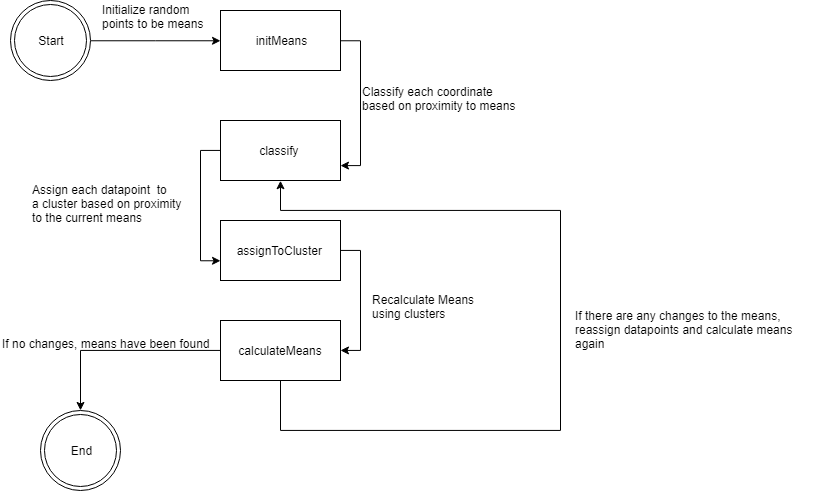
\includegraphics[width=1.0\textwidth]{KMeansSM.png}
\end{figure}

\newpage

The diagram below is the UML State Machine Diagram for KruskalMST.

\begin{figure}[h]
\centering
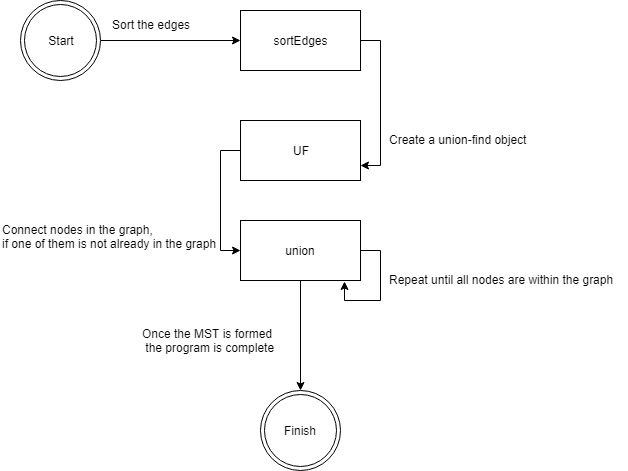
\includegraphics[width=1.0\textwidth]{KruskalSM.png}
\end{figure}

\newpage

\section{Internal Review and Evaluation}

The internal review and evaluation process addresses two important factors of any 
software product: Verification and Validation. We evaluate based on code testing
to verify that the product is working right and review that the right product
is being built by tracing back to specifications, particularly non-functional
specifications, as functional specifications are covered in the modular
decomposition section in more detail.

\subsection{Verification}
\subsubsection{White Box Testing}
For each module, a white box testing procedure is carried out to verify that each
individual components are functioning as expected. Test cases such as boundary 
cases, exception cases and abnormal input are taken into consideration. Each test
case will also obey module interface specification limits and assumptions: For example,
a negative number will not be tested on a function that only accepts $\mathbb{N}$.

\begin{itemize}
\item Cord - Emphasis on constructor, accessor and mutator methods testing.
\item Cluster - Emphasis on constructor, accessor and mutator methods testing.
\item KMeans - Relatively black-boxed approach to testing; Only cluster size verified.
\item Edge - Emphasis on constructor, accessor and mutator methods, as well as comparison
of weights between edges.
\item Graph - Test of properly initialized edges based on points passed into the ADT
\item Heap - Test of proper helper functions, and verification of sorting.
\item UF - Verify union-find  methods are working as expected.
\item KruskalMST - Verify that the constructed MST is optimal.
\item Load - Test that Load functions, and countsort/hash tables are initiated.
\end{itemize}

\newpage

\subsubsection{Black Box Testing}
The modules not included for white box testing in the above section, drawSurface and demoFrame,
are used for black box testing. The purpose is to verify the output given a valid input into
the program. Testing is mainly done on demoFrame as it is the driver of the entire program.
Testing parameters taken into consideration are:

\begin{itemize}
\item Cluster consistency: Since K-Means is a heuristic that randomly selects start points of centroids,
the goal of such a test is to check whether generated cluster hotspots are consistent on each run.
\item Cluster amounts: Since K-Means allows the amount of clusters to be generated to be modified,
several cluster amounts are tested to generate the most consistent and user-friendly output. Too many
clusters may hamper the ability of users to consult the application for its uses, while too few clusters
will provide an inaccurate representation of pickups in the city. Consistency issues are addressed by
testing consistent output for the same amount of clusters.
\item Program runtime: Since the application is intended to be used in real-time, the algorithm and graphical
generation should not exceed a certain threshold, or it may become unusable by its users. This ties to
the requirement that the application should not take more than 3 seconds to complete.
\end{itemize}

\newpage

\subsection {Validation}
The goal of validation is to ensure a correct product, i.e. a product that satisfies requirements, is built.
We evaluate based on non-functional specifications of the product, i.e. software qualities of the
application, and qualify how the project has met each requirement.
\begin{itemize}
\item Reliability: As consistency is constantly emphasized as an important attribute, care is taken
to ensure the algorithm generates similar or equivalent outputs for each run. Steps such as choosing
optimal cluster size is carried out to ensure that consistency is not compromised.
\item Security, Safety, Portability: Out of scope of this project. However, 
if the project scale were to increase, it should be of main concern that the
 platform of this application is secure.
\end{itemize}


\end{document}